\section{Мадэліраванне прататыпа размеркавання патокаў трафіка ў сетках SDN}

У дадзеным раздзеле разглядаецца мадэль невялікай гібрыднай SDN сеткі, якая працуе
пад кантролем вышэапісаннага алгарытма разліку нагрузкі.

Для сімуляцыі сеткі выкарыстоўваецца GNS3 праграма.
GNS3 --- гэта графічны сімулятар сеткі, які дазваляе змадэліраваць віртуальную
сетку з маршрутызатараў і віртуальных машын.

На малюнку \ref{img: model} прадстаўлена мадэль віртуальнай сеткі з 3 маршрутызатараў і 1 кантролера.

\begin{figure}[h!]
    \centering
    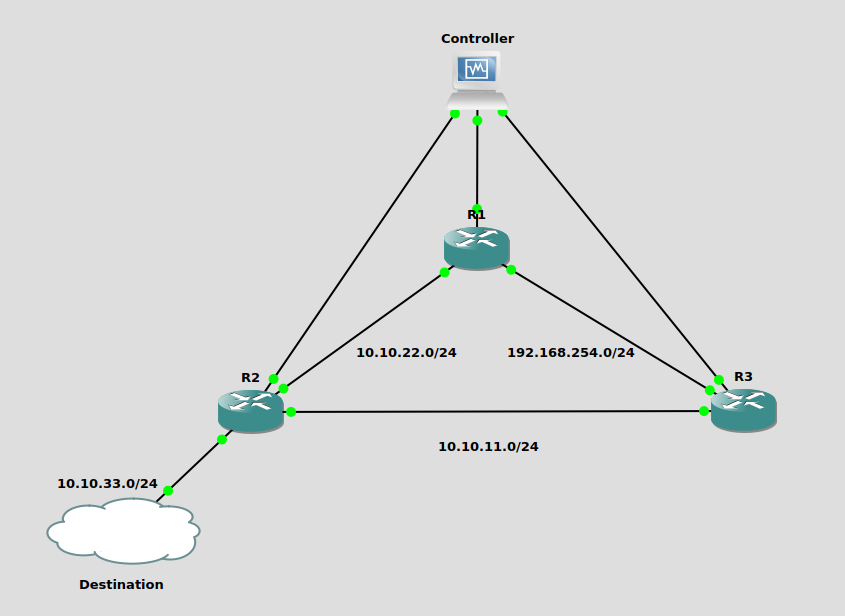
\includegraphics[width=\textwidth]{model.png}
    \caption{Мадэль віртуальнай сеткі}
    \label{img: model} 
\end{figure}

У якасці элемента назірання возьмем маршрутызатар R1 і сеткі 10.10.11.0/24 і 10.10.33.0/24,
так як яны не падключаныя на прамую да выбранага маршрутызатара.

На малюнках \ref{img: initial topology} і \ref{img: initial routers} прадстаўлены
пачатковая тапалогія EIGRP маршрутаў і пачатковыя EIGRP маршруты адпаведна.

\clearpage

\begin{figure}[h!]
    \centering
    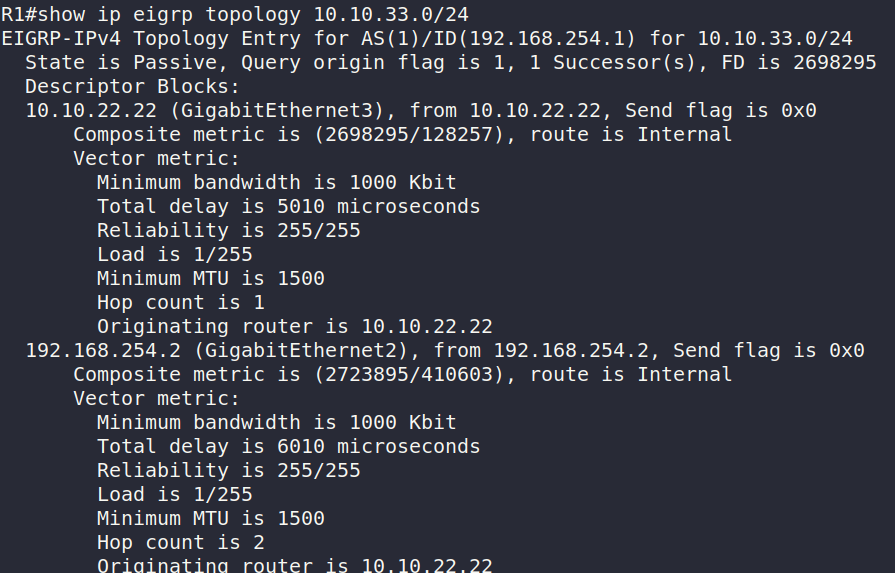
\includegraphics[width=\textwidth]{initial_topology.png}
    \caption{Пачатковая EIGRP тапалогія}
    \label{img: initial topology} 
\end{figure}

\vspace{-\baselineskip}

\begin{figure}[h!]
    \centering
    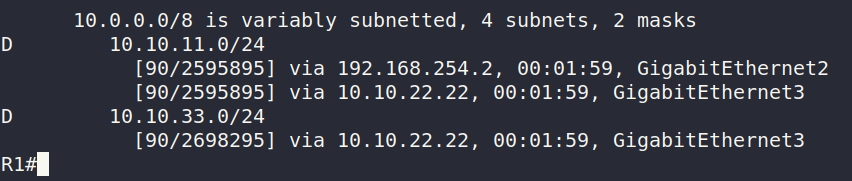
\includegraphics[width=\textwidth]{initial_routes.png}
    \caption{Пачатковыя EIGRP маршруты}
    \label{img: initial routes} 
\end{figure}

Можам заўважыць, што на малюнку \ref{img: initial topology} прадстаўлены 2 магчымых
маршруты да сеткі 10.10.33.0/24, у той час як ў табліцы маршрутызацыі (малюнак
\ref{img: initial routes}) абраны маршрут праз маршрутызатар R2 (адрас інтэрфейса 10.10.22.22). З табліцы маршрутызацыі таксама бачым, што для сеткі 10.10.11.0/24 выкарыстоўваецца балансіроўка паміж 2 маршрутамі.

Для змянення нагрузкі на маршрутызатары R1 будзем выкарыстоўваць тэхналогію flood ping,
якая дазволіць злёгкасцю адпраўляць вялікую колькасць даных за кароткі прамежак часу.
У той жа самы час паралельна запусцім на кантролеры праграму размеркавання патокаў даных для адсочвання нагрузкі.

На малюнку \ref{img: flood ping} прадстаўлена каманда ping.

\begin{figure}[h!]
    \centering
    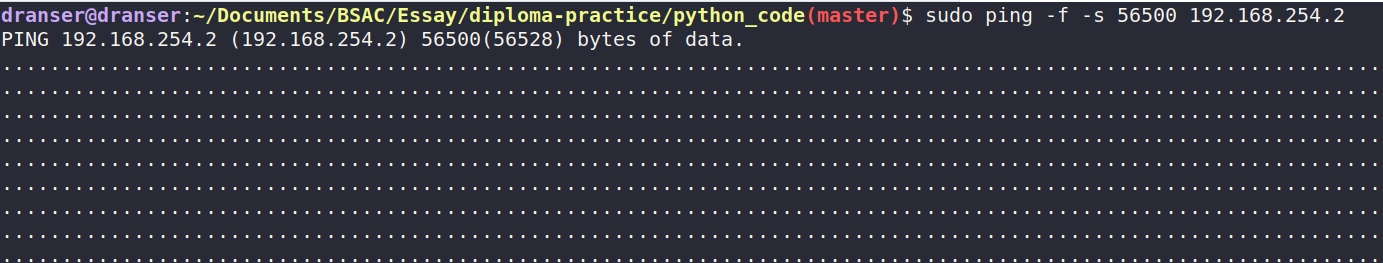
\includegraphics[width=0.5\textwidth]{flood_ping.png}
    \caption{Flood Ping}
    \label{img: flood ping} 
\end{figure}

На малюнку \ref{img: start main} паказаны пачатковы вывад праграмы размеркавання патокаў даных на кантролеры.

\begin{figure}[h!]
    \centering
    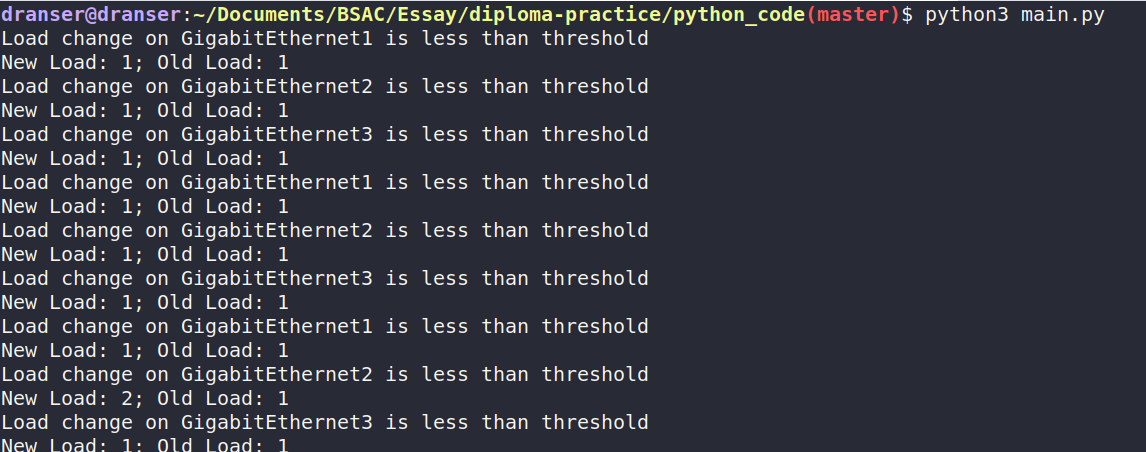
\includegraphics[width=\textwidth]{start_main.png}
    \caption{Пачатковы вывад праграмы размеркавання патокаў}
    \label{img: start main} 
\end{figure}
